\chapter{Binned and binfree analysis of Fluorescence Enhancement by gold nanorod on a 2D layer}
\label{chapter:binfree}
\graphicspath{{./chapters/c3_binfree/img/}}
%============================ MAIN ================================


\begin{abstract}
Gold nanorods are extensively used for single-molecule fluorescence enhancement applications since they are easy to synthesize, bio-compatible and provide high light confinement at their nanometer-sized tips. We report on a novel way to extract the enhancement factor in a single-molecule enhancement experiment using the interphoton delay distribution, avoiding the arbitrary binning of the fluorescence intensity time traces. We present experimental results on the bi-dimensional case, experimentally achieved using a lipid bi-layer to support the diffusion of fluorophores.  We support our findings with a theoretical model to calculate the interphoton delay distribution of (nearly) immobilized emitters from the intensity profile.
\end{abstract}
\newpage

% insert suggested PACS numbers in braces on next line
% \pacs{33.50.Dq,78.67.Qa}
% insert suggested keywords - APS authors don't need to do this
% \keywords{Fluorescence enhancement, TCSPC, Gold-Nanorods}

%\maketitle must follow title, authors, abstract, \pacs, and \keywords
% \maketitle



%%% some explanations
% body of paper here - Use proper section commands
% References should be done using the \cite, \ref, and \label commands
%\section{}

% Put \label in argument of \section for cross-referencing
%\section{\label{}}
%\subsection{}
%\subsubsection{}

% If in two-column mode, this environment will change to single-column
% format so that long equations can be displayed. Use
% sparingly.
%\begin{widetext}
% put long equation here
%\end{widetext}

% figures should be put into the text as floats.
% Use the graphics or graphicx packages (distributed with LaTeX2e)
% and the \includegraphics macro defined in those packages.
% See the LaTeX Graphics Companion by Michel Goosens, Sebastian Rahtz,
% and Frank Mittelbach for instance.
%
% Here is an example of the general form of a figure:
% Fill in the caption in the braces of the \caption{} command. Put the label
% that you will use with \ref{} command in the braces of the \label{} command.
% Use the figure* environment if the figure should span across the
% entire page. There is no need to do explicit centering.

% \begin{figure}
% \includegraphics{}%
% \caption{\label{}}
% \end{figure}

% Surround figure environment with turnpage environment for landscape
% figure
% \begin{turnpage}
% \begin{figure}
% \includegraphics{}%
% \caption{\label{}}
% \end{figure}
% \end{turnpage}

% tables should appear as floats within the text
%
% Here is an example of the general form of a table:
% Fill in the caption in the braces of the \caption{} command. Put the label
% that you will use with \ref{} command in the braces of the \label{} command.
% Insert the column specifiers (l, r, c, d, etc.) in the empty braces of the
% \begin{tabular}{} command.
% The ruledtabular enviroment adds doubled rules to table and sets a
% reasonable default table settings.
% Use the table* environment to get a full-width table in two-column
% Add \usepackage{longtable} and the longtable (or longtable*}
% environment for nicely formatted long tables. Or use the the [H]
% placement option to break a long table (with less control than 
% in longtable).
% \begin{table}%[H] add [H] placement to break table across pages
% \caption{\label{}}
% \begin{ruledtabular}
% \begin{tabular}{}
% Lines of table here ending with \\
% \end{tabular}
% \end{ruledtabular}
% \end{table}

% Surround table environment with turnpage environment for landscape
% table
% \begin{turnpage}
% \begin{table}
% \caption{\label{}}
% \begin{ruledtabular}
% \begin{tabular}{}
% \end{tabular}
% \end{ruledtabular}
% \end{table}
% \end{turnpage}


\section{Introduction\label{sec:intro}}

%Here goes the intro. IDEAS:
%
%- characterization of fluorescence time traces with intensity, blinking, correlation function, histograms of photon counts.
%
%- try to get rid of binning because it introduces an additional arbitrary parameter. Histograms of interphoton times (macrotime delays), similar to histograms of microtime delays used for lifetime determination; more characterization methods, but here focus on interphoton delay histograms
%
%- Here we show that this histogram relates to a distribution of intensities of single molecule fluorescence. Therefore it encodes information about the intensity distribution inside the volume accessible to diffusion. We will assume diffusion uniform in accessible volume.
%
%- Importance for near-field distribution in enhanced fluorescence around plasmonic structures. 
%Will be illustrated here with enhancement of single-molecule fluorescence by gold nanorods with different geometries. 

Single quantum emitters such as fluorophores, quantum dots, color centers 
and fluorescent proteins have become powerful tools for modern science 
since they provide nanometer-sized probes that can be used to extract 
information about the local environment \cite{moerner1999illuminating, kulzer2010single}, 
oxidation state of molecules\cite{zhang2017gold} and proximity of other 
emitters\cite{stein2011single} combined with the non-invasiveness of optical methods. 
%With the blossom of superlocalization and superresolution techniques, optical microscopy commonly pushed to sub-diffraction-limited scales \cite{klar2000fluorescence,betzig2006imaging}. Recent developments have achieved resolutions comparable with molecular sizes \cite{balzarotti2017nanometer,Weisenburger2017}, opening up the possibility of mapping nanoscale properties unprecedented resolution while keeping the advantages of optical microscopy.

%REMIDNER: WRITE the next two paragraphs, ignore now: % this needs to be replaced with the real text
%
%-Importance of single-molecule studies: get full distributions, avoid synchronization, detection of rare events and dynamical heterogeneity in biological process. 

%-Fluorescence enhancement by plasmonic structures paragraph: physical origins, dependence, mention emission and excitation. limitations. motivate the quantification of enhancement in different structures.
Fluorescence enhancement by plasmonic nanostructures has been successfully 
used in the past to increase the signal from weak 
emitters\cite{kinkhabwala2009large, yuan2013thousandfold, khatua2014resonant} even in 
living cells \cite{vanzanten2010imaging}. In a nutshell, fluorescence enhancement
by metallic nanoparticles refers to an increase in the detected 
photon rate from a molecule when it is placed in the vicinity of the nanoparticle.
It relies on the surface plasmon resonance of the nanoparticle, which is accessible
in the optical range. When excited at this resonance frequency, 
the nanoparticles can concentrate optical fields in tiny volumes,
the so-called ''hot-spots'', providing a sub-diffraction 
working volume that can be exploited to perform, for example, 
fluorescence correlation spectroscopy (FCS) at micro molar 
concentrations\cite{estrada2008,manzo2011nanoscale,punj2013gold,khatua2014enhancedfluorescence}.
It can also extend the powerful tools of single-molecule spectroscopy to 
weakly emitting species.


Regardless of the origin of the fluorescence photons, a usual approach is to record the arrival time each individual 
photon in the so-called time-correlated single-photon counting approach (TCSPC) in a time-tagged 
time-resolved configuration (TTTR) \cite{Wahl_picoquant}. 
Thanks to the high-speed electronics and pulsed excitation sources available commercially, 
the absolute arrival times (also called macrotime) can be determined with picoseconds accuracy and, with the proper synchronization to the excitation source, the 'nanotime'\footnote{The usual denomination is microtime but we opt for nanotime to avoid confusion with the macrotime.} can be also determined. 
The nanotime is usually used to obtain the lifetime histogram, which can be used to 
gain insight into the underlying mechanism for the emission. For example, 
in the case of fluorescence, the radiative and non-radiative rates can be accessed experimentally with a 
measurement of the lifetime and the quantum-yield \cite{lakowicz2007principles}.
%Figure \ref{fg:tcspc} shows an time representation for such an experimental configuration. 
The output of a TTTR experiment can be represented as a classical function of time \cite{Lippitz2005}:

\begin{equation}
I(t) = \sum_i \delta( t-t_i)
\label{eq:intensity_TCSPC}
\end{equation}
where $\delta(t)$ is the usual definition for the Dirac's delta function and $t_i$ is the absolute arrival time
for each detected photon in the experiment (measured relative to the start of the experiment, the macrotime). 
We shall call this function \textit{unbinned time trace}. 
 

 %\begin{figure}
 %\includegraphics[width=\textwidth]{img/TCSPC_scheme.pdf}%
 %\caption{\textbf{Time-correlated single-photon counting detection scheme.} Typical configuration for a time-tagged time-resolved photoluminescence experiment. The exciting source is a pulsed laser with MHz repetition rate and both the time tag $T$ since the start of the experiment and the TCSPC time $t$ are recorded and saved. The former can be used to calculate the interphoton delay distribution and the latter to generate a lifetime histogram to obtain, for example, the lifetime of a fluorescent molecule. Modified from \cite{Wahl_picoquant}.
%\label{fg:tcspc}}
 %\end{figure}

In spite of the high temporal resolution provided by such experiments, 
the usual way to characterize the emission of quantum emitters is to 
display the temporal fluctuations of the number of detected photons 
in a certain integration time (or binning time) and
complement this with the histogram of detected photon counts. 
Such a characterization inherently introduces an arbitrary parameter, 
the binning or integration time, that may bias the obtained distribution\cite{Lippitz2005}. 
Alternatively, correlation functions can be calculated from the unbinned
 time trace to exhibit the characteristic 
time of a process of interest, such as the diffusion time of molecules
in solution\cite{magde1972thermodynamic,haustein2007fluorescence} and 
other molecular properties even at single molecule level \cite{medina2002fluorescence}.

Here we focus on the use of a less common quantity the 
\textit{interphoton delay distribution} $p(\tau)$
to characterize the emission of quantum emitters and to extract reliable 
information about an emitting system avoiding the introduction of any arbitrary 
binning time. The interphoton delay distribution express the delay distribution 
between photons: after a photon detection, the probability density to observe 
the next photon at a time $\tau$ is $p(\tau)$ ($p(\tau)\geq 0$) \cite{Verberk2003}.
We present a model to relate this quantity to a distribution of intensities probed by a 
single quantum emitter in the limit of \textit{slow} diffusion and we show that it 
encodes information about the intensity distribution inside the volume accessible 
to diffuser. We will illustrate this point with single-molecule fluorescence 
in a bi-dimensional case both with Gaussian beam shape and in the case of 
enhanced fluorescence using gold nanorods.


\section{Theoretical framework}

We seek to relate the interphoton delay distribution in a fluorescence experiment with 
the spatial distribution of intensities used to excite the fluorescent molecules. The interphoton
delay distribution was defined above and is represented by the probability density function $p(\tau)$. 
Thus the probability of detecting the next photon at a time 
$\tau+\mbox{d}\tau$ is $p(\tau)\mbox{d}\tau$ and the
normalization condition holds: $\int_0^{\infty}{p(\tau)\mbox{d}\tau}=1$.

Let us start from the simplest case of a constant detected intensity $w$ 
(in counts per second). Such a signal gives rise to an exponentially distributed 
interphoton delay times, i.e., 
\begin{equation}
p(\tau)=w\exp(-w\tau)\,.
\label{eq:exponential_distribution}
\end{equation}
This is a direct consequence of the memory-free character of the photon 
emission, which leads to a Poisson distribution of intensities and an 
exponential distribution of interphoton delays. We note that this distribution 
can be obtained with a fluorescent molecule excited at a constant intensity, 
for example, a fixed molecule on a substrate excited at a constant intensity. 

Let us now consider a distribution of intensities $Q(w)$ such that the 
intensity variations are much slower than the interphoton detection events.
This will give rise to the interphoton delay distribution 
$p(\tau)=\int_0^\infty w e^{-w\tau}Q(w)\mbox{d}w$ that corresponds to 
averaging over all possible intensities (rates) $w$ and can be rewritten as

\begin{equation}
p(\tau)=-\frac{\mbox{d}}{\mbox{d}\tau}\mathscr{L}\{Q(w)\}(\tau)\,,
\label{eq:interphoton_delay_distribution}
\end{equation} 
where $\mathscr{L}\{Q(w)\}(\tau)=\int_0^\infty e^{-w\tau}Q(w)\mbox{d}w$ denotes the 
Laplace transform of the function $Q(w)$ \footnote{Note that the Laplace transformation
is usually applied to time-dependent functions, giving rate-dependent functions. 
Here, we apply it to a function of the rate to obtain a time-dependent transform.}. 
If we would like to obtain the interphoton delay distribution 
corresponding to an addition of two sources with intensity distributions $P(w)$ 
and $Q(w)$ we can use the total intensity $T(w)$ that can be calculated as the sum 
of a combined probability of soruce 1 emitting at a rate $x$ and sorce 2 a 
$(w-x)$, i.e., by convoluting the two intensity functions: $T(w)=\int{P(x)Q(w-x)\mbox{d}x}$. 
Using the convolution theorem we can write the Laplace transform of the intensity distribution 
as the product of the Laplace transforms of the two distributions, from which we can deduce 
the interphoton delay distribution.

Let us now consider as a source one emitting object at position $\ve{r}$ 
diffusing around an optical intensity maximum, for example, a fluorescent molecule. 
The detected intensity will generally be a product of the position-dependent local 
excitation intensity and of a position-dependent collection efficiency and the 
molecular parameters involved in the emission process (absorption cross section, 
fluorescence quantum yield, etc. ). We write the product of these factors as a 
position-dependent intensity function $I(\ve{r})$. 

At this point we make two important approximations to continue. The first one is 
to neglect rotational diffusion of the molecules, which is a good approximation 
if we study times that are much longer than the rotational diffusion time. The 
second important approximation is to assume that translational diffusion is slow
 compared to the photon detection rate, that is to say, the molecules are fixed 
during the emission process. A complete theory relaxing this approximations would 
be much more complicated to develop and it is outside the scope of this work.

Under this approximations, the photon distribution can be deduced from the 
intensity distribution. The exploration of the diffusion volumes by the moving 
object gives rise to the following distribution of intensities 
\begin{equation}
Q_1(w)=\frac{1}{V}\int_V{\delta\left( w-I(\ve{r})\right)\mbox{d}^3r} \,,
\label{eq:intesity1}
\end{equation} 
where $\delta(x)$ represents the Dirac delta function and $V$ the volume 
accessible by the molecule. In order to calculate the interphoton delay 
distribution using equation \ref{eq:interphoton_delay_distribution} we should 
compute the Laplace transform of $Q_1(w)$. This transformation results in 
\begin{equation}
\mathscr{L}\{Q_1(w)\}(\tau) = 1 -\lambda(\tau) \quad \mbox{where} \quad 
\lambda(\tau)\equiv \frac{1}{V}\int_V{ \{1-\exp[-I(\ve{r})\tau]\}\mbox{d}^3r} \, .
\label{eq:one-emitter}
\end{equation} 
Note that, for an intensity variation with a finite range around the center, 
for example due to Gaussian illumination and collection, $\lambda(\tau)$ is a 
small quantity which tends to zero for a large diffusion volume.  

We now consider the case of many ($N$) emitters with a concentration $C=\frac{N}{V}$
 diffusing in a large volume. Using the argument presented before for two emitters, 
the addition of one emitter will modify the intensity distribution by convolution 
with the one-emitter distribution function $Q_1(\tau)$. Using the convolution theorem 
for the Laplace transform, we can write the Laplace transform for the $N+1$ diffusers as
\begin{equation}
\mathscr{L}\{Q_{N+1}(w)\}(\tau) = \mathscr{L}\{Q_N(w)\}(\tau) \mathscr{L}\{Q_1(w)\}(\tau)\,,
\label{eq:laplace_N}
\end{equation}
from which we deduce 
$\mathscr{L}\{Q_{N}(w)\}(\tau)=\left[\mathscr{L}\{Q_{1}(w)\}(\tau)\right]^N $. 
Now we apply the statistical method of Stoneham \cite{STONEHAM1969, Fleury1995} 
by letting number and volume tend to infinity keeping the ratio constant to match 
the concentration $C$ to approximate
\begin{equation}
\ln\left[\mathscr{L}\{Q_{N}(w)\}(\tau)\right] = 
N\ln\left[1-\lambda(\tau)\right] \approx - C V \lambda(\tau)\,.
\label{eq:stoneham_approx}
\end{equation}

Therefore, using this result in equation \ref{eq:interphoton_delay_distribution} 
together with the definition from equation \ref{eq:laplace_N}, the general result 
for the histogram of interphoton delays for a concentration $C$ of emitters diffusing 
in a intensity maximum described by $I(\ve{r})$ 
\begin{equation}
p(\tau)=-\frac{\mbox{d}}{\mbox{d}\tau}\left[ 
\exp\left(-C \int_V{\left(1-\exp\left[-\tau I(\ve{r})\right] \right)}
\mbox{d}^3\ve{r}    \right)\right]\,.
\label{eq:result}
\end{equation}

This is a general result that allows us to calculate the interphoton 
delay histogram  for a solution with a concentration $C$ of (slowly) 
freely-diffusing objects around an illumination profile $I(\ve{r})$. 

\subsection{Photons per burst distribution}

Still need to revisit the theory and contrast with the experimental results.

%\subsection{Diffusion case}
%
%What happens if we add diffusion. Add qualitatively arguments of how the distribution is changed. mention the very fast
%diffusion limit: it is a single exp. In the middle we have to say how we expect it to look.

\section{Two \textit{constant} different intensities}

In order to show that we can avoid the binning of our TTTR data to 
extract valuable information about our experiment, we studied the 
simple case of two constant detected intensities. In such a scenario, 
the interphoton delay distribution will be a biexponential function.

\begin{figure}
\centering
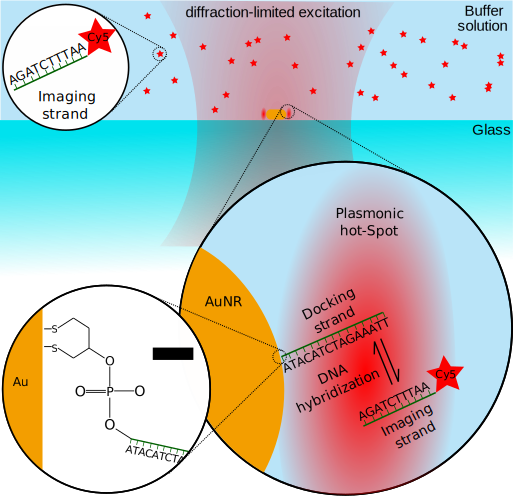
\includegraphics[width=0.6\textwidth]{Transient_scheme}%
\caption{\textbf{Transient binding experimental scheme.} We used a 
home-made confocal microscope to excite and detect the imaging 
strand-Cy5 constructs in the solution. The signal from the molecules 
in the solution is low, thus we enhance the fluorescence signal using 
immobilized gold nanorods on a glass surface (average size: 45$\times$90 nm). 
In order to experimentally access the same spatial position in the plasmonic 
hot-spot we use the transient binding technique with a 15 base pair-long 
DNA as a docking strand and a 10base-pair-long imaging strand. 
The docking strand is attached to the gold nanorod surface using 
two tiol bonds, as shown in the inset. More details about the sample 
preparation can be found in the supplementary information. 
\label{fg:transient}}
\end{figure}

We experimentally access this situation by using fluorescence enhancement
by individual gold nanorods. In such a scenario, 
a 1000-fold intensity enhancement can be achieved for weak 
dyes\cite{yuan2013thousandfold,khatua2014resonant}. However, this enhancement value
depends strongly on the position of the molecule in the nanosale plasmonic 
hot-spot of the structure \cite{khatua2014resonant}, thus the challenge in 
such experiments is to place the dye molecules in the desired position to 
achieve high enhancement values. An elegant solution to place the molecules 
in the desired position is the technique called transient binding \cite{acuna2012fluorescence}.
Briefly, we use two complementary single-stranded DNA sequences, one attached
 to the surface of a gold nanorod and the other one is marked with a single Cy5
 molecule (fluorescence quantum yield 0.27). The strand attached to the gold 
surface is  called the docking strand, since it allows the complementary strand 
to dock in one specific site and the latter is called the imaging strand since 
it allows fluorescence detection. 

This experimental scheme is shown in figure \ref{fg:transient}. We immobilized 
a gold nanorod on a glass surface and we have the imaging strands diffusing 
freely in the buffer solution. Details on the sample preparation can be found 
in the Supplementary Information. When an imaging strand diffuses close to the 
docking strand, the DNA can be hybridized, forming a temporary double strand DNA. 
In that scenario, the single fluorescent label is placed in the plasmonic 
hot-spot of the nanorod and gets enhanced, giving a higher signal than the 
other molecules in the detection volume. 
This approach allows to put a single dye in a well-defined position in the 
near-field of the nanorod for a exponentially distributed time whose 
mean value can be selected with the length length of the DNA and the 
environment conditions \cite{}. Since the dye molecule is fixed at a 
certain point in space, with a fixed exciting intensity, we expect a 
fixed detected intensity. The main advantage of this experimental 
approach is that the hybridization is transient and after some time 
the DNA will de-hybridize, freeing the docking site for another 
imaging strand to come. As a result, photobleaching of the dye 
is not a limiting factor for the experiment, since \textit{the same point} 
in space can be probed several times with different single molecules.

\begin{figure}
\centering
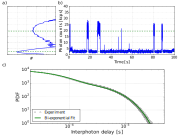
\includegraphics[width=0.95\textwidth]{transient_single_site_results}
\caption{\textbf{Fluorescence enhancement of single Cy5 molecules with transient binding.}
(a) Binned intensity histogram. (b) Binned fluorescence time trace (bin time = 1 ms). 
From these two plots, two intensity levels are clearly recognized: the high 
level corresponds to the enhanced fluorescence signal of one Cy5 molecule at 
a fixed position in the hotspot while the low level corresponds to the 
intensity from gold nanorod luminescence plus the contribution of the 
un-enhanced molecules in the detection volume (free docking-strand, 
shown in the inset on the right).
(c) Interphoton delay probability density function (PDF) obtained 
from the TTTR measurements (empty dots) and a biexponential fit, one 
for each intensity level. The retrieved intensities from this fit are 
shown in green dashed lines in (a) and (b), which coincide with the 
high and low levels.
\label{fg:transient_results}}
 \end{figure}



Figure \ref{fg:transient_results} shows the experimental results
 on our two-intensity system. On plot (a), at the top left, we 
show the typical characterization of the fluorescence time traces, 
a binned time trace which shows the evolution in time of the 
number of counts and on the right the histogram of binned 
intensity. Two levels can be clearly identify, the high-fluorescence 
level corresponds to the inset in (a), the DNA docking strand and 
imaging strand are hybridized and a dye molecule is kept at a fixed 
position in the hotspot, thus emitting enhanced fluorescence. After 
some seconds the DNA de-hybridizes and the imaging strand leaves the 
hot-spot, thus the signal goes down. 
The low level signal can be attributed to the luminescence of the 
gold nanorod and of the unenhanced molecules in the confocal volume. 
For our purpose here, we have a detected stream of photons coming 
from two well-defined intensity levels. 
We would like to retrieve these two levels using the interphoton 
delay distribution by fitting a biexponential function. 
Figure \ref{fg:transient_results} (c) shows the experimental curve 
and the fitting, from which we extracted the intensity levels 
marked in (a) and (b) with dashed lines. These levels clearly 
reproduce the levels evidenced by the binned time trace and intensity 
histograms, but they were obtained without the need of any arbitrary 
parameter. In the supplementary material we show how the binned plots 
change dramatically with the binning time. 

The results in this simple case show how useful this type of analysis 
can be, since we were able to extract information from our TTTR data 
without introducing any arbitrary parameter.


\section{Gaussian beam in two dimensions\label{sec:gaussian2d}}

A more realistic scenario to use our analysis is the problem of two 
dimensional diffusion of fluorescent molecules around a Gaussian beam, 
described by an intensity function $I(\ve{r}) = I_0 \exp[-r^2/\sigma^2]$, 
where $(r,\theta)$ are the normal polar coordinates in the plane and 
$\sigma$ represents the waist of the beam. 
In this case, the intensity profile is bi-dimensional and only depends
on the distance to the center of the beam and we take a concentration 
$C$ of fluorescent molecules per unit area. Using this intensity 
distribution in equation \ref{eq:result} we calculate the expected 
interphoton delay distribution $p_G(\tau)$and find the integral form
\begin{equation}
p_{G}(\tau)=-\frac{\mbox{d}}{\mbox{d}\tau}\left[ \exp\left(-C \sigma_0^2 \pi \int_{\epsilon}^1\left(1-\exp\left[-\tau I_0 u \right]\right) \frac{\mbox{d}u}{u}\right)    \right]\,,  
\label{eq:gaussian2d}
\end{equation}
where we defined $\epsilon \equiv \exp\left(-\frac{R^2}{\sigma^2}\right)$ 
and $R$ is the maximum radius accessible by the diffusing molecules.

We studied this case experimentally in a regular confocal microscope 
by confining the diffusion of ATTO647N dye molecules in a lipid bi-layer, 
obtaining a bi-dimensional case and a reduced diffusion coefficient of 
$D=4.4\, \mu$m$^2$s$^{-1}$, as presented previously\cite{pradhan2016goldnanorodenhanced}. 

\begin{figure}
\centering
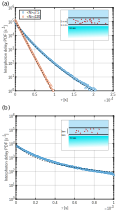
\includegraphics[width=0.5\textwidth]{2D_gaussian_with_single}%
\caption{\textbf{Bidimensional molecular diffusion probed with a Gaussian beam.} 
(a) Interphoton delay probability density function (PDF) for the case 
of high concentration of molecules, with an average
number of molecules $<N>=7.5$ or $120$ in the detection area 
$A=\pi\sigma^2$ (corresponding to $\approx 14$ and $225$ molecules 
per $\mu$m$^2$, respectively). The circles with error bars are 
experimental values while the green solid line is 
the fit with the model from equation \ref{eq:gaussian2d}. 
A good agreement is found. (b) Interphoton delay probability 
density function (PDF) for the case of low concentration
of molecules, $<N>=0.5$ ($\approx 0.9$ molecules per $\mu$m$^2$). 
In this case we find some deviations
from the theory. 
\label{fg:gaussian2d}}
\end{figure}

We performed the experiment for high and low concentrations 
of molecules in the lipid bi-layer and fitted 
the experimental interphoton curves with $p_{G}(\tau)$ from 
equation \ref{eq:gaussian2d} using the experimental value 
for the beam waist, $\omega_0=292$ nm. 
Figure \ref{fg:gaussian2d} shows the experimentally obtained interphoton 
delay probability density function for high (a) and low (b) concentrations 
along with the corresponding fits using our theoretical result. 
In the case of high concentration the model reproduces the results quite 
well while for the low concentration it does not. This is a direct 
consequence of the main approximation in our model, that neglects the 
effect of diffusion, which can be applied for the case of many molecules 
in the Gaussian focal spot but fails in the case of low number of molecules. 
The deviations found could be used to study diffusion. We also note that 
the higher the number of molecules, the more exponential
the curve looks. This is consistent with the limit of extremely high 
number of molecules, discussed in the appendix. 
% BIS: be careful, remove this last line

\section{Model for the enhancement in two dimensions}

We now turn to the case of plasmonic enhancement. We first use present 
a semi-analytical approach with simple 
intensity distributions that mimic the complicated process of fluorescence 
enhancement by metallic nanoparticles to 
gain some intuition on the behavior of the impact that these effect has in 
the interphoton delay distribution.
The simple model we take for the near-field intensity distribution is the 
sum of a Gaussian beam
and a radial power law with exponent $\alpha$: 
\begin{equation}
I(r) = W_0 \left[ \exp \left(-\frac{r^2}{\sigma^2} \right) + E \left(\frac{R_{NP}}{r}\right)^\alpha  \right]\,, 
\quad r \leq R_\textrm{NP}
\label{eq:enhancement_model}
\end{equation}
where $W_0$ is the unenhanced intensity, $\sigma$ the width of the Gaussian 
illumination, $E$ the enhancement
factor and $R_\textrm{NP}$ the nanoparticle radius. 
We note that the Gaussian case studied in the previous section is re-obtained for $R_\textrm{NP}=0$. Figure
\ref{fg:enahncement_model} (a) shows the comparison of this intensity distribution for two different values 
of the exponent $\alpha$ with the unenhanced case. 
With this intensity spatial distribution we calculated the interphoton delay distribution by numerically 
solving the integral in \ref{eq:result}. Note that the area inside the nanoparticle is not accessible
to the molecules so the integration was carried from $r=R_\textrm{NP}$.
The obtained distributions are shown in figure \ref{fg:enahncement_model} (b) 
for a $10$ molecules in the Gaussian area.  Clearly the distributions with enhancement show a more peaked feature at
extremely short interphoton times due to the high rate emission created when a molecule enters the 
enhanced intensity area in the near-field. 

In order to quantitatively compare the interphoton delay distributions for the different cases we decided to 
fit the curve with a stretched exponential, i.e. we use the function
\begin{equation}
f(\tau) = A \exp\left( \lambda \tau^\beta\right)
\label{eq:strechted_exp}
\end{equation}
to approximate the complicated behavior of the interphoton delay distribution. This works reasonably for short 
times and fails to reproduce the tails in the curves. Nevertheless, we focus our analysis in the short times
which contain the information of the enhancement. We fit the calculated PDFs for different concentrations of molecules
ranging from the situation of a very diluted sample ($10^{-2}$ molecules in the Gaussian area given by $\pi \sigma^2$) to an extremely high number of molecules ($10^{6}$). Figure \ref{fg:enahncement_model} (c) shows the obtained exponent for
different concentrations for the three cases mentioned. In the Gaussian case we approximate to the exponential case
$\beta=1$ for $<N>=100$ while for the enhanced case we need 3 orders of magnitude higher concentration. This is
in agreement with the fact that the ratio of the near field area $A_\textrm{NF}$
(consider as the volume that contains intensities highers than $EW_0\exp(-1)$) to the far field $A_\textrm{FF}=\pi\sigma^2$ is $\frac{A_\textrm{NF}}{A_\textrm{FF}} \sim 10^{-3}$. In other words, to obtain an 
exponential-like interphoton delay distribution we need to completely fill with molecules the near field area. 




\begin{figure}
\centering
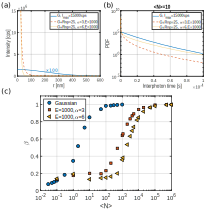
\includegraphics[width=0.9\textwidth]{enhancement_model}%
\caption{\textbf{Simple model for plasmonic enhancement  in two dimensions.} (a) Radial intensity distributions for Gaussian (blue solid line, multiplied by 100 for display), $\alpha=3$ (red dashed line) and $\alpha=6$ (yellow dotted line). 
For all the cases the intensity is $W_0=1.5\times10^4$ and the enhancement factor is $E=1000$.
(b) Interphoton delay probability density function (PDF) for the three cases presented in (a).
(c) $\beta$ from the stretched exponential fit.
\label{fg:enahncement_model}}
\end{figure}



\section{Gold nanorod with molecules in two dimensions}


Re-visit biswajit paper results: instead of cherry picking we give an average value more representative and bin-free.

Methods:

Cherry pick

binned intensity histogram slope

interphoton times


 %\begin{figure}
 %\includegraphics[width=0.8\textwidth]{img/Enhancement_interphoton_1.pdf}%
 %\caption{\textbf{Gold nanorod for fluorescence enhancement in bidimensional diffusion.} .
%\label{fg:enhancement}}
 %\end{figure}


\section{Conclusions}

In this paper we characterized single-molecule fluorescence traces 
from a variety of experimental conditions with the \textit{interphoton
delay distribution} to avoid the arbitrary introduction of a binning time. 
We show with some examples that this quantity is an useful tool to characterize
a stream of photons, specifically when there is enhancement.

We presented an analytical model for the case of slowly diffusing molecules that
allows the calculation of interphoton delay distribution from the spatial intensity 
distribution.With this model we could reproduce the main features of molecules diffusing 
in a lipid bi-layer when they are illuminated with a Gaussian beam.
%=========== Supporting info ========
\newpage
\section{Supporting Info}
\graphicspath{{./chapters/c3_binfree/si_figure/}}

\section*{Transient Binding sample preparation}


\section*{Binned time traces dependence with bin time}



\section*{Lipid bilayer sample preparation}



\section*{2D Numerical simulations}

The current program is organized in only one script, simualtion2d.m and contains several subroutines. It also uses the program generate\_simulation\_parameters.m to set all the needed parameters for the simulation. These are divided in two sets, the physical parameters and the simulation parameters. 
The former set of parameters corresponds to the experimentally relevant variables while the latter corresponds to the extra parameters needed to run the simulation and are not related to the experimental conditions but need to be selected to run the simulation. 
The output of the program is a structure that has contains the unbinned time traces, binned time traces and interphoton histograms. The physical inputs are the following: concentration of molecules $C$, intensity distribution of the incoming beam $I(\ve{r})$ and dark counts of the detector $Dc$. 
For a complete list of the simulation parameters, refer to the appendix \ref{ap:sim_param}.

The calculation consists of several steps that will be summarized in the following. 
The spatial intensity distribution input has to be a matrix $M$ with the spatial intensity distribution of the incoming beam $I(\ve{r})$ (in cps). 
The first step is done by the subroutine \texttt{calculate\_times} to simulate the absolute arrival photon times for each intensity value of the matrix 
\footnote{This can be improved in speed by not calculating the repeated intensity values more than one time and by saving the output structure in a file and loading it later instead of recalculating it.} 
within the time of the experiment, $T_{\mbox{Max}}$. This traces correspond to a single molecule placed in each pixel of the intensity matrix.
To generate the correct exponential distribution for a given intensity $I$, I use the fact that the interphoton times should follow an exponential distribution:
\begin{equation}
\Delta t_{i} = -\frac{\log\left(\zeta_i \right)}{I} \, ,
\label{eq:interphoton_simulation}
\end{equation}
where $\Delta t_{i}$ ($i=0,...,N$) represents the time between successive photons detection and $\zeta_i$ is a random number in the interval $(0,1)$. 
This way of generating the interphoton times ensures the required exponential distribution. Then by performing the cumulative sum over the interphoton times the absolute arrival times of the simulated stream of photons can be calculated for each intensity value in the input intensity matrix $M$. This data is contained in a structure named \texttt{abs\_times}. 

The next step is to calculate the number of molecules present in the simulation volume  $V_{sim}$. For a given concentration, the number of molecules contributing to the simulation is random variable that follows Poisson distribution with a mean value $\left<N_{molecules}\right> = C V_{sim}$. Since our calculation is based on the calculation of the interphoton arrival time for a fixed number of molecules $N_{molecules}$ in the simulation volume, we calculate the number of molecules needed to contain 99\% of the cases. Then, for each $N_{molecules}$ we generate the interphoton histogram as follows. We generate random positions for all the available molecules in the simulation volume and we retrieve the corresponding absolute photon arrival times from the variable abs\_times. We concatenate all this arrival time and also include extra photon detections generated by the dark counts of the detector. The mean number of dark photons in the simulation time is $Dc T_{\mbox{max}}$ and follows a poisson distribution. We use a poissonian number generator to simulate the number of detected photons in each run and then distribute them uniformly in the time trace. All this concatenated absolute photon detection times are then sorted and saved in a vector $t$. Then the histogram of the interphoton times for this vector is computed, using pre-fixed bins (with a certain number of points $Hist_{\mbox{Npts}}$) . The normalized (to the total counts) histogram is stored into the first component of a matrix of histogram counts $H$. Then we repeat this procedure $N_{\mbox{config}}$ time, using each time a new set of random positions for all the molecules, creating the matrix of dimensions $Hist_{\mbox{Npts}} \times N_{\mbox{config}}$. Then we average the normalized histograms corresponding to different spatial configurations, contained in $H$ to obtain a single histogram corresponding for a single number of molecules in the simulation volume. The final step is to perform a weighted average of the histograms for each number of molecules contributing to the simulation for a fixed concentration using the corresponding poissonian weight.



\section*{Slow diffusion case}

We simulated the case of a molecule 


\section*{Simulation Parameters\label{ap:sim_param}}

\section*{code validation\label{ap:code}}

In order to validate the simulation code we tested the results with a simple beam shape that provides an analytical solution. 
We work in two dimensions just for simplicity with a rectangular beam shape with constant intensity and zero intensity outside, described mathematically as:
\begin{equation}
I(x,y) = I_0\theta(|x-\frac{x_0}{2}|)\theta(|y-\frac{y_0}{2}|)\, ,
\label{eq:theta_intensity}
\end{equation}
with $I_0$ the maximum intensity and $x_0,y_0$ the size in lateral directions and $\theta(\zeta)$ the step function. Thus, the illuminated area has a volume of $V_0=x_0y_0$. 
For such a beam shape the interphoton probability distribution can be obtained by simple integration of equation \ref{eq:result} replacing the beam shape $I(\ve{r})$ with equation \ref{eq:theta_intensity}, obtaining
\begin{equation}
p(\tau) = I_0 C V_0 \exp[-\tau I_0-C V_0(1-\exp(-\tau I_0))]\,.
\label{eq:theta_interphoton_distribution}
\end{equation}

Figure \ref{fg:square_beam}(a) shows an example in a particular case when the dimensions are the same for the two directions and \ref{fg:square_beam}(b) shows plots for the analytical solution for different intensities and concentrations.




 \begin{figure}
 \centering
 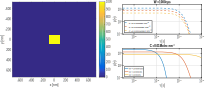
\includegraphics[width=\textwidth]{square_illumination}%
 \caption{\textbf{Simple illumination profile that provides an analytical solution to test the simulation code} 
(a) Colormap plot of the square-shaped beam we use for validating the code. We used $x_0=y_0=182$ nm and $I_0=1000$ cps.
(b)Analytical plots of the interphoton probability distribution for different intensities and concentrations. 
\label{fg:square_beam}}
 \end{figure}


%\figdouble{square_illumination}{square_illumination_analytical}{fg:square_beam}{Simple illumination profile that provides an analytical solution to test the simulation code}{ \figa Colormap plot of the square-shaped beam we use for validating the code. We used $x_0=y_0=182$ nm and $I_0=1000$ cps. \figb }


In order to test the code we performed simulations using this illumination distribution and compared it with the analytical result. We started with a fixed superficial concentration  C=$2 \times 10^{-4}$ molecules nm$^2$ to have a relative fast run and we changed the different parameters of the simulation, such as the number of spatial configurations to average and the total simulation time $T_{\mbox{max}}$. The comparison with the analytical curves can be seen in figure \ref{fg:sim_test}. In both cases the simulation agrees well with the analytical result and for longer simulation time or higher number of configurations, the error becomes smaller.


 \begin{figure}
 \centering
 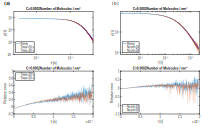
\includegraphics[width=\textwidth]{Theta_results}%
 \caption{\textbf{Test of simulation parameters and code validation} 
(a) Different total simulation times. Top: simulated and analytical curves. Bottom: relative error in the simulation.
(b) Different number of averaged spatial configurations. Top: simulated and analytical curves for different total simulation times $T_{\mbox{max}}$. Bottom: relative error in the simulation.
\label{fg:Theta_results}}
 \end{figure}


The next step was to test the simulation for different physical parameters such as the concentration of molecules and the intensity in the beam. The results for three different concentrations and intensities can be found in figure \ref{fg:phy_test}. The results again agree with the analytical curves and it can be noted that the larger the number of photons generated in the simulation the better correspondence with the analytical result.


 \begin{figure}
 \centering
 \includegraphics[width=\textwidth]{Theta_physical_test}%
 \caption{\textbf{Test of physical parameters and code validation} 
(a) Different concentrations. Top: simulated and analytical curves. Bottom: relative error in the simulation.
(b) Different intensities. Top: simulated and analytical curves. Bottom: relative error in the simulation.
\label{fg:Theta_physical_test}}
 \end{figure}}